\section{Stolpersteine}

Bei der Berechnung der Welle mittels Potenzreihen gibt es mehrere Dinge die 
beachtet werden m"ussen. Von besonderer Signifikanz sind vor allem die 
Genauigkeit der L"osungen f"ur die jeweilien $x$, sowie der nat"urlich auch die 
Zeit die f"ur die Berechnung ben"otigt wird.


\subsection{Genauigkeit}
Gem"ass
\begin{equation*}
	y(x) = a_0 + a_1x 
	-\sum_{k=2}^{\infty}\frac{1}{k(k-1)}(aa_{k-4}+ba_{k-3}+ca_{k-2})x^k
\end{equation*}
m"usste man f"ur jedens $x$ eine unendliche Anzahl Additionen ausf"uhren. Was 
aber bedeuted, dass die Berechnung f"ur ein einzelnes $x$ unendlich lange 
dauern w"urde. Folglich muss man die maximale Anzahl $k$ einschr"anknen.

\begin{equation*}
	y(x) = a_0 + a_1x 
	-\sum_{k=2}^{k_{\text{max}}}\frac{1}{k(k-1)}(aa_{k-4}+ba_{k-3}+ca_{k-2})x^k
\end{equation*}

Das hat aber weitreichende Folgen. So wird je nach $k_{\text{max}}$ fr"uher 
oder sp"ater die L"osungswerte gegen $\infty$ oder $-\infty$ gehen. Das liegt 
daran, dass der Term $(x - x_0)^k$ einer finiten Reihe um die 
Entwicklungsstelle $x_0$, je weiter sie sich von diesem entfernen, gegen"uber 
den $a_k$ beginnen wird zu dominieren.

Die folgende Graphik zeigt auf wie die L"osung der Gleichung 
\ref{eq:wellen:grundgleichung} mit verschiedenen $k_{\text{max}}$ aussieht.

\begin{center}
	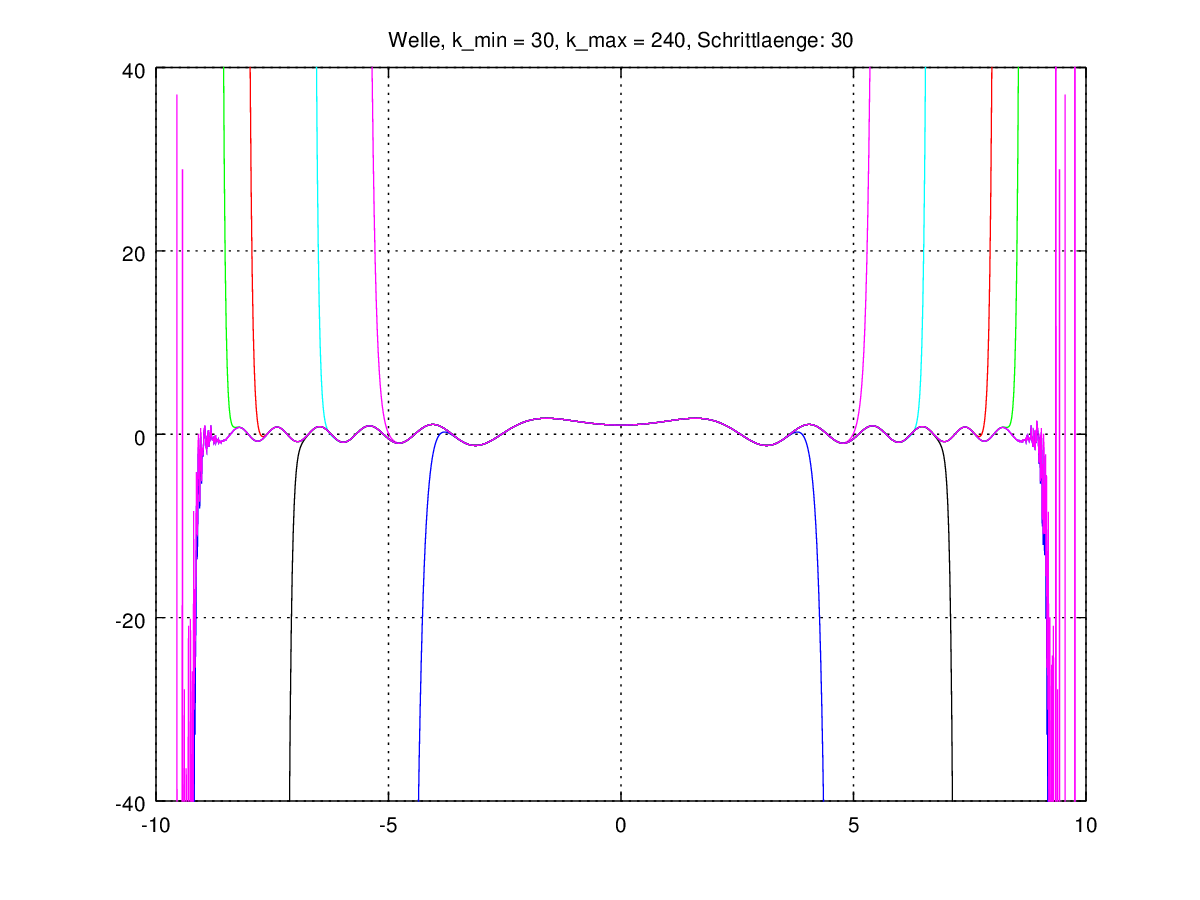
\includegraphics[scale=0.65]{./wellen/images/kmax/krangewaveeven.png}
\end{center}

Es ist leicht zu erkennen, das mit gr"osser werdenen $k$ auch der Punkt an dem 
$x^k$ dominiert sich weiter von $x_0$ entfernt. Es taucht noch ein weiteres 
Ph"anomen auf. Da die Werte von $a_k$ immer kleiner werden und die von $x^k$ 
immer gr"osser, kommt der Rechner irgendwann an seine Grenzen und beginnt 
unbrauchbare Resultate zu liefern. Diese Ungenauigkeit ist durch die bin"are 
Repräsentation von Dezimalzahlen und den limitierungen der verschiedenen 
Datentypen wie \texttt{double} oder \texttt{float} in einem Rechnersystem 
gegeben.

\subsection{Berechnungszeit}
Die Berechnung von Potenzreihenl"osung im Intervall
$[x_{\text{min}},x_{\text{max}}]$ kann "ausserst lange dauern. Auch hier kann
muss Anzahl Berechnungen, in diesem Fall die Aufl"osung des Plots,
eingeschr"ankt werden. Eine genauere Absch"atzung kann mit Hilfe des
Pseudocodes \ref{alg:wellen:potenzreihenrechnung} gemacht werden.

\begin{algorithm}
	\floatname{algorithm}{Pseudocode}
	\begin{algorithmic}[1]
		\State $a_{-2} \gets 0$
		\State $a_{-1} \gets 0$
		\State $a_0 \gets y(0)$
		\State $a_1 \gets y'(0)$
		\State $k \gets 2$
		\State $x \gets x_{\text{min}}$
		\For{$x \le x_{\text{max}}$}
			\State $k \gets 2$
			\State $\text{sum} \gets a_0 + a_1x$
			\For{$k \le k_{\text{max}}$}
				\State $a_k \gets -\frac{1}{k(k-1)}			
				(aa_{k-4}+ba_{k-3}+ca_{k-2})$
				\State $\text{sum} \gets \text{sum} + a_k x^k$
				\State $k \gets k + 1$
			\EndFor
			\State $x \gets x + x_{\text{step}}$
		\EndFor
	\end{algorithmic}
	\caption{Wellen Potenzreihenberechnung} 
	\label{alg:wellen:potenzreihenrechnung}
\end{algorithm}

Der Algorithmus hat also eine Laufzeit von
\begin{equation*}
	\mathcal{O}\left(k_{\text{max}}\frac{x_{\text{max}}-x_{\text{min}}} 
	{x_{\text{step}}}\right).
\end{equation*}
